\chapter{Findings \& Analysis}
\label{ch:findings}

This chapter presents our findings, organized along the retrieval-to-citation pipeline: from search trigger and query generation, through source overlap with conventional search engines, to structural content preferences and citation fidelity.

%-----------------------------------------------------------------------
\section{ChatGPT Search Trigger}
\label{sec:fanout}
\label{sec:search-trigger-section}

When a user sends a message, ChatGPT must first decide whether to search the web at all. This section examines how that decision is made, based on the classifier metadata we extracted from the network event stream.

\label{sec:search-trigger}
\label{sec:three-layer}

All of the following observations come from the raw network event stream that ChatGPT sends to the browser during response generation (Section~\ref{sec:chatgpt-anatomy}, Figure~\ref{fig:network-response}). Before ChatGPT generates anything, a classifier called the Sonic Classifier runs.
 Its job is to decide whether the question needs fresh web data or whether the model can answer from its training knowledge.
  It runs once when the user sends a message.

A previous classifier version (\texttt{sonic\_force\_pg\_switcher}), documented by \textcite{resoneo2026chatgpt} and \textcite{williamscook2025sonic}, used a single probability and a single-step decision:

\begin{enumerate}
    \item If \texttt{search\_prob} $> 0.65$, trigger a simple search. Otherwise, answer from training knowledge.
\end{enumerate}

\noindent The classifier's configuration, including its thresholds, is sent as part of the network event stream alongside every response---this is how we were able to extract them.

\noindent The model would only search if it was confident that we need a search triggered. 
The version we observed (\texttt{sonic\_classifier\_5p2\_3cls\_ev3}, model \texttt{snc-pg-sw-3cls-ev3}), identical across both Business and Personal tiers throughout our data collection window (January~2026), worked a little differently. 
It outputs three probabilities---\texttt{simple\_search\_prob}, \texttt{complex\_search\_prob}, and \texttt{no\_search\_prob}---that sum to 1.0, and evaluates them in a fixed order:

\begin{enumerate}
    \item If \texttt{no\_search\_prob} $\geq 0.175$, suppress search (answer from training knowledge).
    \item Else if \texttt{complex\_search\_prob} $\geq 0.4$, trigger a complex search (never observed in our data; its exact behavior is unknown).
    \item Else trigger a simple search (threshold = 0, so this is the catch-all).
\end{enumerate}

\noindent Search is now the default---it is only suppressed if \texttt{no\_search\_prob} crosses the 17.5\% gate. The system no longer asks ``should I search?'' but ``should I \emph{not} search?'' This likely reflects the trajectory toward treating web grounding as the norm (Section~\ref{sec:reasoning-models}).

Table~\ref{tab:classifier-examples} shows the three probabilities for selected prompts. No prompt in our dataset crossed the 0.4 complex-search threshold, so all classified runs were routed to simple search.

\begin{table}[H]
\centering
\caption{Sonic Classifier probabilities for selected prompts. The three values sum to 1.0 and are deterministic for a given prompt.}
\label{tab:classifier-examples}
\small
\begin{tabular}{@{}p{5.2cm}rrr@{}}
\toprule
\textbf{Prompt (ID)} & \textbf{simple} & \textbf{complex} & \textbf{no\_search} \\
\midrule
What are direct competitors of Doctranslate that offer similar services? (P046) & .694 & .295 & .011 \\
Can you recommend the best free AI TTS software with celebrity voices for IoT? (P053) & .736 & .259 & .005 \\
What is the best machine translation tool for live translation that saves context? (P063) & .955 & .037 & .008 \\
I need live transcribing while using online streaming or watching videos. (P016) & .792 & .034 & .174 \\
What are some free AI tools for audio transcription? (P022) & .997 & .0002 & .003 \\
\bottomrule
\end{tabular}
\end{table}

Table~\ref{tab:search-trigger-breakdown} summarizes the search trigger outcomes across all 474 ChatGPT runs. The high search rate is expected given that our prompts are commercial product queries---exactly the kind of question that benefits from fresh web data.

\begin{table}[H]
\centering
\caption{Search trigger breakdown across 474 ChatGPT runs (79 prompts $\times$ 3 runs $\times$ 2 tiers).}
\label{tab:search-trigger-breakdown}
\small
\begin{tabular}{@{}lrrr@{}}
\toprule
 & \textbf{Business} & \textbf{Personal} & \textbf{Total} \\
\midrule
\multicolumn{4}{@{}l}{\emph{Run-level outcomes (237 runs per tier)}} \\
\quad Search triggered & 218 (92.0\%) & 214 (90.3\%) & 432 (91.1\%) \\
\quad No search & 19 (8.0\%) & 23 (9.7\%) & 42 (8.9\%) \\
\midrule
\multicolumn{4}{@{}l}{\emph{Prompt-level consistency (79 prompts, across all 6 runs)}} \\
\quad Always searched (6/6) & \multicolumn{2}{c}{} & 70 \\
\quad Never searched (0/6) & \multicolumn{2}{c}{} & 6 \\
\quad Mixed & \multicolumn{2}{c}{} & 3 \\
\bottomrule
\end{tabular}
\end{table}

\noindent The six prompts that never searched tend to be phrased as general how-to questions---e.g.\ \emph{``How can I convert an audio file to text?''} (P013)---for which the model answered entirely from training knowledge and produced few or no citations.

Only three prompts showed mixed behavior. The clearest case is P016 (\emph{``I need live transcribing while using online streaming or watching videos.''}): on Business, all three runs searched; on Personal, none did. Its \texttt{no\_search\_prob} of .174 sits just 0.001 below the 0.175 suppression threshold---same prompt, different tier, opposite outcome. The classifier configuration and thresholds are identical across tiers, so the divergence occurs somewhere downstream. P004 and P045 also showed within-tier variation---searching in 2 of 3 runs on the same tier---but this was rare (2 of 79 prompts).


When search was triggered, we observed \texttt{web.run} tool calls in the event stream issuing pairs of reformulated queries---the fan-out queries discussed in the next section. As of late February~2026, the \texttt{sonic\_classification\_result} block (classifier ID, thresholds, and probabilities) is no longer exposed in the event stream; the search decision now happens entirely server-side. The underlying Sonicberry model (\texttt{alpha.sonic\_thinky\_v1\_paid}) remains identical to our January data collection period and is still visible in the stream (Figure~\ref{fig:sonicberry}), as are \texttt{web.run} calls and fan-out queries.

\begin{figure}[H]
\centering
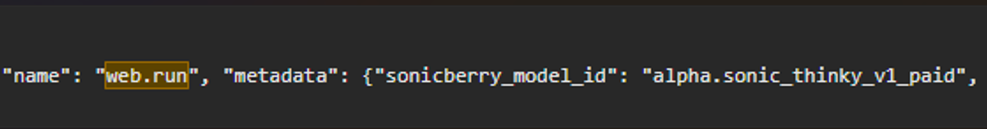
\includegraphics[width=\textwidth]{figures/sonic_berry.png}
\caption{A \texttt{web.run} tool call from the network event stream, showing the \texttt{sonicberry\_model\_id} in the metadata block.}
\label{fig:sonicberry}
\end{figure}

\section{Fan-Out Queries}
\label{sec:fanout-queries}
\label{sec:freshness-steering}

Once the search decision is made, the model reformulates the user's prompt into search engine queries, commonly called \emph{fan-out queries}. For example, when a user asks \emph{``What are some free AI tools for audio transcription?''} (P022), ChatGPT issues two queries:

\begin{quote}
\small
\texttt{Q1:} free AI tools for audio transcription\\
\texttt{Q2:} best free speech to text transcription tools online
\end{quote}

\noindent The first query closely mirrors the user's prompt; the second rephrases it with synonyms and broader terms, widening the retrieval pool (see Figure~\ref{fig:fanout-raw} for how these appear in the raw network stream). Across all runs, the three environments produced 2{,}280 fan-out queries: 448 from Business, 424 from Personal, and 1{,}408 from Gemini. ChatGPT issues exactly two queries per search turn, though it occasionally triggers additional turns (Section~\ref{sec:multi-turn}). Gemini exposes 3--7 queries per run in its grounding metadata.

\subsection{Multi-Turn Re-Search}
\label{sec:multi-turn}

In 12 of 432 searched runs (across 5 prompts), the model evaluated its first-round results, 
then issued a second (or third) \texttt{web.run} call with new queries. 
First-round queries are generic fan outs of the user prompt, while later rounds target specific products discovered in the initial results (Table~\ref{tab:multi-turn-queries}).
\begin{table}[H]
\centering
\caption{Multi-turn query content for ChatGPT re-search runs.}
\label{tab:multi-turn-queries}
\small
\begin{tabular}{lrp{3.8cm}p{4.5cm}}
\toprule
Prompt & Turns & Turn 1 Queries & Turn 2+ Queries \\
\midrule
P035 & 2 & ``translation services with live interpreters pricing\ldots'' & ``Jeenie live interpreter pricing per minute\ldots'', ``Jeenie or Boostlingo pricing'' \\
P053 & 2 & ``free AI text to speech celebrity voices\ldots'' & ``ElevenLabs free tier celebrity voices API IoT\ldots'', ``open source TTS celebrity voices or voice cloning\ldots'' \\
P050\_r3 & 2 & ``free app live translation during a call French\ldots'' & ``Google Translate app live conversation translation\ldots'', ``Microsoft Translator app real time voice\ldots'' \\
P073\_r3 & \textbf{3} & ``best video translator for YouTube\ldots'' & Turn 2: ``tools to translate YouTube videos subtitles or audio\ldots''; Turn 3: ``tools like VEED, Kapwing, Happy Scribe'' \\
\bottomrule
\end{tabular}
\end{table}

Gemini's grounding metadata does not expose separate turns, but the query sequence suggests the same pattern. In P002\_r1, for example, Q1--Q2 are generic reformulations of the prompt (\emph{``AI text to speech multi-speaker dialogue tools 2025''}, \emph{``best text to speech services for multi-voice conversations''}), while Q3--Q7 each target a specific brand discovered from those initial results: Murf~AI, ElevenLabs, Speechify, Play.ht. The progression from broad category queries to narrow brand queries mirrors ChatGPT's multi-turn re-search, suggesting that Gemini evaluates its first-round results and issues follow-up queries for individual products---it is just not exposed as discrete turns.

\subsection{Year Injection in Fan-Out Queries}
\label{sec:freshness-subsection}

Gemini systematically injects year tokens into its fan-out queries. For the same prompt (P006, \emph{``What are the best apps or AI tools to transcribe audio to text?''}), ChatGPT searched for \emph{``apps or AI tools to transcribe audio to text''} and \emph{``best speech-to-text transcription tools AI''}---no year token. Gemini's raw grounding metadata for the same prompt shows year tokens in every query:

\begin{lstlisting}[language=json,numbers=none]
"webSearchQueries": [
  "AI tools for transcribing long audio files 2026",
  "best AI audio to text transcription tools 2025 2026",
  "best free audio transcription apps 2026",
  "highest accuracy AI transcription services 2026"
]
\end{lstlisting}

This is not an isolated case. 96.7\% of Gemini runs (297/307 with valid grounding metadata) include at least one year-injected query, and 66.8\% of all individual Gemini queries (940/1{,}408) contain a year token. Figure~\ref{fig:gemini-year-serp} shows what this produces on the SERP side: searching for one of these year-injected queries returns almost exclusively year-tagged listicles (``11 Best AI Transcription Apps\ldots\ in 2026,'' ``The 3 Best Transcription Services of 2026,'' etc.). This means Gemini's citations are biased toward this kind of content---pages with the current year in their title or headings are far more likely to match these queries and enter the retrieval pool.

\begin{figure}[H]
\centering
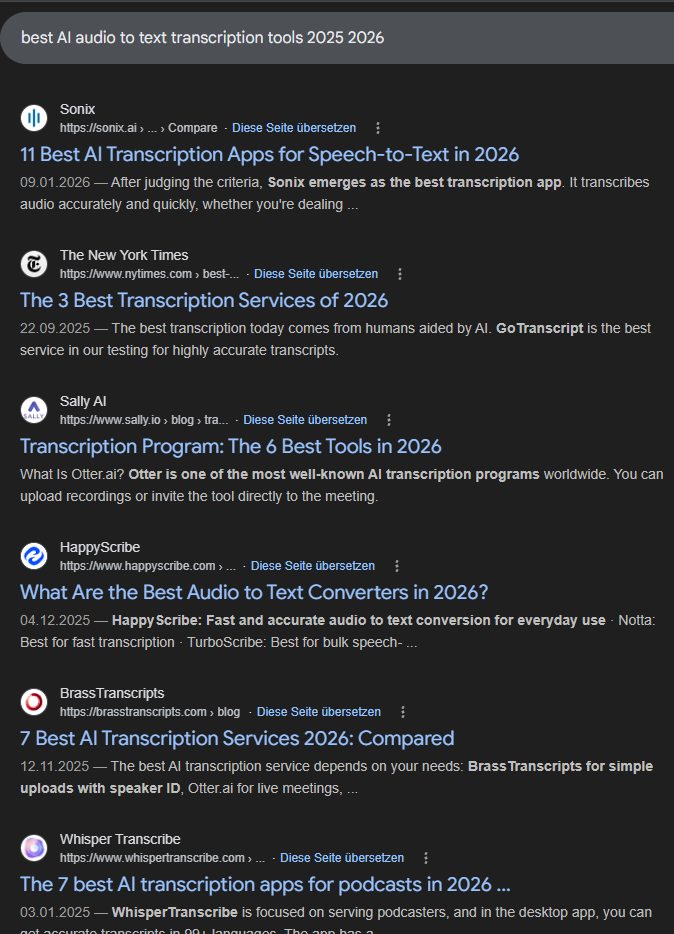
\includegraphics[width=0.75\textwidth]{figures/serp_fanout.png}
\caption{Google SERP for Gemini's year-injected query \emph{``best AI audio to text transcription tools 2025 2026''}.
 Nearly every result is a year-tagged listicle.}
\label{fig:gemini-year-serp}
\end{figure}
ChatGPT also occasionally injects year tokens, but only in 5.1\% of runs. Its freshness preferences are discussed in Section~\ref{sec:selection-drift}.

\subsection{Cross-Language Fan-Out}
\label{sec:localization-bias}

OpenAI documents that ChatGPT ``collects general location information
 based on your IP address and may share that general location with 
 third-party search providers'' \parencite{openai2024searchhelp}. 
 A user in Munich who asks ``best bakery'' will see the fan-out rewritten 
 to ``best bakery near Munich Germany''---the location is injected directly into the query text. We call this \textbf{explicit localization}.

Our software dataset has no local-commerce queries that would trigger explicit localization, but we observed something we call \textbf{implicit localization}. When this same user in Munich asks ``best free website to translate a video and add subtitles,'' the response text is in English---yet many of its citations point to German web pages. This happens because one fan-out is issued in English and the other in German, routing half the retrieval into the 
German-language search index without the user ever seeing it. This observation was one of the reasons we routed all data collection through a US-based proxy (Section~\ref{sec:proxy-requirement}).

Across our GPT runs we identified three patterns of implicit localization, all orchestrated through fan-out queries invisible to the end user.

\subsubsection{Case~1: Foreign Prompt $\rightarrow$ English Fan-Out}

When the user searches in a non-English language, GPT pairs a fan-out in the user's language with one in English. For example, P019 (\emph{``Quel est le meilleur logiciel de traduction instantan\'{e}~?''}) produces:

\begin{quote}
\small
\texttt{Q1:} meilleur logiciel de traduction instantan\'{e}e traduction en temps r\'{e}el logiciel\\
\texttt{Q2:} best real-time translation software instant translation tools comparison
\end{quote}

\noindent Of the 7 foreign-language prompts in our dataset, 5 triggered web search; all 5 produced this pattern on every run (\textbf{30/30 = 100\%}). The remaining two (Italian, Spanish) were answered from training knowledge without triggering search at all.

This is corroborated at scale by \textcite{rudzki2026english}, who analyzed over 10~million prompts and 20~million query fan-outs from Peec~AI's production monitoring data. They report that \textbf{78\%} of non-English ChatGPT sessions include at least one English-language sub-search, and \textbf{43\%} of all fan-out queries for non-English prompts target the English web---consistent with our 100\% rate.

Gemini shows a variation of this pattern. For foreign-language prompts, it always 
reserves the first grounding query slot (which is the strongest fan out, Section~\ref{sec:per-query-citation}) for an English translation of the prompt.

\subsubsection{Case~2: Context-Triggered Local-Language Fan-Out}

When the prompt is in English but mentions a foreign language---either explicitly in the text or implicitly through IP/locale signals---GPT sometimes pairs the English fan-out with one in a local language. Unlike Case~1's near-universal trigger, Case~2 is selective: whether it fires depends on how central the foreign language is to the user's intent.

\begin{itemize}
    \item P058 ``best software for Parsian/Farsi audio-to-text transcription'' $\rightarrow$ Farsi fan-out on every run (tool must work \emph{in} Farsi)
    \item P050 ``free app for\ldots a call with French speakers'' $\rightarrow$ French fan-out on some of the runs only (since user themselves might not necessarily be speaking French)
    \item P026 ``transcribe Spanish videos into English'' $\rightarrow$ never triggered (foreign language is just the input source)
\end{itemize}

\subsubsection{Case~3: Untriggered Cross-Language Fan-Out}
\label{sec:untriggered-cross-lang}

The most surprising pattern: \textbf{24 runs} across 15 English-language prompts received non-English fan-outs despite containing no foreign-language signal whatsoever. This includes prompts about translation tools (e.g., P018 ``Can you suggest a free website or program that can translate my 20-minute video and add subtitles?'' $\rightarrow$ Chinese fan-out), but also prompts with no connection to language at all:

\begin{itemize}
    \item P016 ``I need live transcribing while using online streaming'' $\rightarrow$ Chinese fan-out
    \item P017 ``Can you recommend a text to speech service\ldots'' $\rightarrow$ Japanese fan-out
    \item P048 ``Can I add a live translation app to calls?'' $\rightarrow$ Spanish fan-out
    \item P031 ``Are there currently any free audio to text transcription services?'' $\rightarrow$ Japanese fan-out
\end{itemize}

\noindent Nothing in these prompts explains why the model would search in Chinese or Japanese. Unlike Case~2, where the prompt at least mentions a foreign language, here the prompt gives no signal at all.

Case~3 also shows cross-run instability: the same prompt can produce different target languages across runs. 
P018 (``Can you suggest a free website or program that can translate my 20-minute video and add subtitles?'') 
received non-English fan-outs on 4 of 6 runs, switching between Chinese (enterprise), 
Japanese (enterprise), and Spanish (personal); P048 (``Can I add a live translation app to calls?'') triggered on 3 of 6, 
alternating between Japanese (enterprise) and Spanish (personal). 

\subsubsection{GEO Takeaways on Localization}
 
A website targeting only French speakers historically did not need to account for localization. 
But for AI visibility, even if this website is well optimized for SEO and ranks high in French search results for relevant keywords, it is still competing against the entire English web for half of its AI visibility. To unlock the other half, the publisher would have to
 localize their site and build an SEO strategy for English keywords, which will often be far more competitive and require more investment.

The reverse also holds: Cases~2 and~3 show that English-language prompts can produce localized fan-outs. A website ranking well in English search results might still lose potential visitors in Germany because ChatGPT, based on the user's IP address or simply the nature of the conversation, decided to issue a French or German fan-out instead.

These findings show that a true multi-lingual SEO approach is almost a prerequisite for GEO.

%-----------------------------------------------------------------------
\section{Citation Origins}
\label{sec:position-bias}
\label{sec:citation-overlap}


\subsection{Index Affinity: Which Search Engine?}
\label{sec:global-overlap}

For each LLM citation, we checked whether the exact URL appeared in our Bing or Google SERP scrape for 
the same fan-out queries that produced it.
The most significant finding is that the search index behind ChatGPT's citations depends a lot on the subscription tier.

\begin{table}[H]
\centering
\caption{Global citation overlap by provider and subscription tier}
\label{tab:global-overlap}
\small
\begin{tabular}{@{}lrrr@{}}
\toprule
 & \makecell[r]{GPT\\Business} & \makecell[r]{GPT\\Personal} & Gemini \\
\midrule
Total Cited Links & 1,637 & 1,839 & 1,651 \\
Total Additional Links & 2,820 & 4,506 & --- \\
Total Rejected Links & 631 & 496 & --- \\
Bing Overlap (Cited) & \textbf{81.3\%} & 67.6\% & --- \\
Bing Overlap (Additional) & \textbf{86.3\%} & 56.3\% & --- \\
Google Overlap (Cited) & 27.8\% & \textbf{64.6\%} & \textbf{77.7\%} \\
Google Overlap (Additional) & 20.7\% & 52.1\% & --- \\
\midrule
Total Index Coverage & 83.7\% & 80.6\% & 77.7\% \\
Invisible (neither index) & 16.3\% & 19.4\% & 22.3\% \\
\bottomrule
\multicolumn{4}{l}{\scriptsize Coverage: Business/Personal = Bing $\cup$ Google; Gemini = Google only.}
\end{tabular}
\end{table}


Across all three tiers, \textbf{78--84\%} of citations trace back to a conventional search index. 
This confirms that traditional search ranking is the dominant factor for AI visibility. The remaining 16--22\% (the ``invisible'' share) is another element that makes GEO distinct from SEO,
 and we examine it in Section~\ref{sec:invisible-links}.

GPT Business states that it retrieves exclusively through its official partner, the Bing Search API \parencite{openai2024enterprise}, and our data confirms this: 81.3\% Bing overlap versus only 27.8\% Google. Even when an LLM does not retrieve from a given engine, some overlap is expected because there are only so many websites that cover a given topic. Any search engine searching for the same keywords will end up returning many of the same pages. We treat that 27.8\% as the natural overlap that comes from this shared relevancy pool.

GPT Personal jumps to 64.6\% Google overlap, a 36.8\,pp
increase over that baseline, while its Bing overlap drops to 67.6\%.
This suggests that the Personal tier retrieves from Google alongside Bing, which aligns with OpenAI's documentation referring to ``third-party search providers'' in the plural \parencite{openai2024search}. Citation matches against Google SERP features (Table~\ref{tab:serp-feature-matches}) support this: Personal shows roughly double the PAA matches of Business (44 vs 23). Since these features are Google-specific, the disparity is another indicator that Personal retrieves from Google more heavily.

\begin{table}[H]
\centering
\caption{Citation matches against Google SERP features.}
\label{tab:serp-feature-matches}
\begin{tabular}{lrr}
\toprule
Feature & GPT Business & GPT Personal \\
\midrule
People Also Ask (PAA) & 23 & 44 \\
Video & 3 & 3 \\
Discussion & --- & 3 \\
\bottomrule
\end{tabular}
\end{table}

For publishers, this means that optimizing only for Bing (as many would think) or Google is not 
enough for ChatGPT visibility. Just as the cross-language fan-out findings (Section~\ref{sec:localization-bias}) 
showed that an English website is a prerequisite even for non-English audiences, the index affinity 
data shows that Bing rankings matter for ChatGPT especially for Business-tier users
A brand that ranks well on Google but has no Bing presence may be effectively invisible to the largest ChatGPT deployment tier.

\subsection{Overlap Distribution by SERP Position}
\label{sec:page-dist}
\label{sec:bing-page-dist}
\label{sec:google-page-dist}

Match counts below combine cited links (URLs that appear in the final response) and additional links (URLs that ChatGPT retrieved but did not surface to the user; see Section~\ref{sec:chatgpt-anatomy}).

\begin{figure}[H]
\centering
\begin{subfigure}[t]{0.48\textwidth}
\centering
\begin{tikzpicture}
\begin{axis}[
    ybar,
    bar width=8pt,
    width=\textwidth,
    height=6cm,
    ylabel={Matches},
    xlabel={Bing Page},
    ymin=0,
    ymax=1600,
    xtick={1,...,16},
    xticklabel style={font=\scriptsize},
    yticklabel style={font=\scriptsize},
    ylabel style={font=\small},
    xlabel style={font=\small},
    title style={font=\small\bfseries},
    title={GPT Business -- Bing},
    fill=entcolor,
    draw=entcolor!80!black,
]
\addplot coordinates {
    (1,1468) (2,333) (3,656) (4,692) (5,641)
    (6,560) (7,453) (8,437) (9,312) (10,271)
    (11,248) (12,202) (13,191) (14,166) (15,140) (16,103)
};
\end{axis}
\end{tikzpicture}
\caption{Business on Bing: clear Page~1 spike.}
\label{fig:bing-business-dist}
\end{subfigure}
\hfill
\begin{subfigure}[t]{0.48\textwidth}
\centering
\begin{tikzpicture}
\begin{axis}[
    ybar,
    bar width=8pt,
    width=\textwidth,
    height=6cm,
    ylabel={Matches},
    xlabel={Bing Page},
    ymin=0,
    ymax=700,
    xtick={1,...,16},
    xticklabel style={font=\scriptsize},
    yticklabel style={font=\scriptsize},
    ylabel style={font=\small},
    xlabel style={font=\small},
    title style={font=\small\bfseries},
    title={GPT Personal -- Bing},
    fill=perscolor,
    draw=perscolor!80!black,
]
\addplot coordinates {
    (1,521) (2,345) (3,663) (4,602) (5,667)
    (6,579) (7,590) (8,480) (9,433) (10,426)
    (11,391) (12,327) (13,293) (14,286) (15,264) (16,204)
};
\end{axis}
\end{tikzpicture}
\caption{Personal on Bing: flatter profile.}
\label{fig:bing-personal-dist}
\end{subfigure}

\vspace{1em}

\begin{subfigure}[t]{0.48\textwidth}
\centering
\begin{tikzpicture}
\begin{axis}[
    ybar,
    bar width=5pt,
    width=\textwidth,
    height=6cm,
    ylabel={Matches},
    xlabel={Google Rank},
    ymin=0,
    ymax=180,
    xtick={1,3,5,7,9,11,13,15,17,19,21,23,25,27,29},
    xticklabel style={font=\scriptsize},
    yticklabel style={font=\scriptsize},
    ylabel style={font=\small},
    xlabel style={font=\small},
    title style={font=\small\bfseries},
    title={GPT Personal -- Google},
    fill=perscolor,
    draw=perscolor!80!black,
]
\addplot coordinates {
    (1,168) (2,128) (3,145) (4,107) (5,112)
    (6,113) (7,103) (8,92) (9,48) (10,38)
    (11,58) (12,57) (13,65) (14,41) (15,48)
    (16,50) (17,38) (18,46) (19,23) (20,29)
    (21,30) (22,21) (23,39) (24,27) (25,18)
    (26,14) (27,22) (28,16) (29,6)
};
\end{axis}
\end{tikzpicture}
\caption{Personal on Google: top-rank concentration with Page~2 bump.}
\label{fig:google-personal-dist}
\end{subfigure}
\hfill
\begin{subfigure}[t]{0.48\textwidth}
\centering
\begin{tikzpicture}
\begin{axis}[
    ybar,
    bar width=5pt,
    width=\textwidth,
    height=6cm,
    ylabel={Matches},
    xlabel={Google Rank},
    ymin=0,
    ymax=200,
    xtick={1,3,5,7,9,11,13,15,17,19,21,23,25,27,29},
    xticklabel style={font=\scriptsize},
    yticklabel style={font=\scriptsize},
    ylabel style={font=\small},
    xlabel style={font=\small},
    title style={font=\small\bfseries},
    title={Gemini -- Google},
    fill=gemcolor,
    draw=gemcolor!80!black,
]
\addplot coordinates {
    (1,181) (2,105) (3,93) (4,92) (5,70)
    (6,62) (7,72) (8,51) (9,39) (10,21)
    (11,24) (12,26) (13,22) (14,23) (15,21)
    (16,20) (17,22) (18,18) (19,22) (20,14)
    (21,7) (22,11) (23,13) (24,9) (25,7)
    (26,15) (27,11) (28,0) (29,2)
};
\end{axis}
\end{tikzpicture}
\caption{Gemini on Google: rank-1 spike with gradual decay.}
\label{fig:google-gemini-dist}
\end{subfigure}
\caption{Citation match distribution by SERP position. Each chart uses its own Y-axis scale.}
\label{fig:overlap-dist}
\label{fig:bing-page-dist}
\label{fig:google-rank-dist}
\end{figure}

The Page~2 dip on both Bing charts is consistent with the pagination
instability documented in Section~\ref{sec:bing-pagination-instability}.
Page~1 leads in match count for Business despite returning a median of only
3 organic results (Table~\ref{tab:bing-page1-size})---with a full 10-result page,
the spike would likely be substantially larger showing how much importance ChatGPT 
gives to Bing first page results.
Matches remain steady through Pages~3--8 and even at Page~16 we do not fully converge---yet
the gradual decline shows that an underlying ranking signal persists.
To put this in perspective: comparing cumulative match counts, Bing Pages~3--16
cover roughly the same information as Google ranks~5--29.
The flatter distribution on Bing is indicative of how noisy the consumer UI pagination is,
and the Bing overlap charts should be seen as a proxy rather than a direct ranking signal.

On Google, the overlap distribution looks much more like we would expect from a Top~30 SERP.
Personal's top ranks (1--8) show the highest concentration, with a notable dip at
ranks 9--10 (48 and 38 matches) followed by an increase at ranks 11--13 (58, 57, 65)---the
top of what would be Page~2 in a standard 10-result SERP.
This mirrors a well-documented pattern in human search behavior: the bottom of Page~1
receives less attention than the top of Page~2.
Seeing this pattern in an AI citation overlap distribution is unexpected, and hints that
how LLMs pick results from SERPs has strong parallels with human behavior.
Gemini on Google shows a similar shape, reinforcing that this positional bias is not
specific to one LLM.

\subsection{Rank Concentration: LLMs vs.\ Human Click-Through}
\label{sec:gemini-google-rank}
\label{sec:cross-system-rank}

For each unique citation URL per run, we find the highest rank at which that URL appears on Page~1 of its corresponding search index (Bing for GPT Business, Google for Gemini, best of both for GPT Personal). Each citation is counted once at its best rank, mirroring how human CTR is measured: of all selections, what share went to each rank? The comparison is restricted to Page~1: on Google, 28.7\% of Personal citation matches fall beyond rank~10, 
so the table captures rank preference Page~1, not overall reliance on it. We clearly can tell that LLMs look deeper than humans do, 
but we include this comparison regardless because the parallel in positional bias between human and LLM behavior is noteworthy.

Table~\ref{tab:cross-rank-ctr} places this LLM rank concentration alongside Google organic click-through rates reported by First Page Sage \parencite{firstpagesage2026ctr}.

\begin{table}[H]
\centering
\caption{Page-1 rank concentration: LLM citation share vs.\ human CTR \parencite{firstpagesage2026ctr}.}
\label{tab:cross-rank-ctr}
\label{tab:cross-rank-concentration}
\label{tab:ctr-comparison}
\begin{tabular}{lrrrr}
\toprule
Rank & Human CTR & \makecell[r]{GPT\\Business} & \makecell[r]{GPT\\Personal} & Gemini \\
\midrule
\textbf{1} & \textbf{39.8\%} & \textbf{24.9\%} & \textbf{26.7\%} & 23.0\% \\
2 & 18.7\% & 24.0\% & 17.5\% & 13.4\% \\
3 & 10.2\% & 13.7\% & 13.5\% & 11.8\% \\
4 & 7.2\% & 9.2\% & 11.4\% & 11.7\% \\
5 & 5.1\% & 7.7\% & 9.1\% & 8.9\% \\
6 & 4.4\% & 6.0\% & 7.2\% & 7.9\% \\
7 & 3.0\% & 5.3\% & 5.8\% & 9.2\% \\
8 & 2.1\% & 4.0\% & 4.4\% & 6.5\% \\
9 & 1.9\% & 3.3\% & 2.6\% & 5.0\% \\
10 & 1.6\% & 1.8\% & 1.8\% & 2.7\% \\
\midrule
Top-3 & 68.7\% & 62.6\% & 57.8\% & 48.2\% \\
\bottomrule
\end{tabular}
\end{table}

All three LLMs show a top-rank preference with a similar decay shape to human click-through behavior, but flatter: top-3 shares range from 48.2\% (Gemini) to 62.6\% (GPT Business) versus 68.7\% for human clicks. GPT Business shows the strongest rank-1 signal (24.9\%), while Gemini is the flattest---its citations spread more evenly across ranks 1--8.

\subsection{Per-Query Citation Distribution}
\label{sec:per-query-citation}

Since both systems issue multiple fan-out queries per run, we checked whether citations are drawn evenly across them or concentrated in one. For ChatGPT, which typically issues two fan-out queries per run, overlap is nearly identical between the two queries across all tiers (Table~\ref{tab:gpt-per-query}). Neither query consistently dominates; citations are drawn from both equally.

\begin{table}[H]
\centering
\caption{GPT per-query citation overlap (474 fan-out queries per tier).}
\label{tab:gpt-per-query}
\begin{tabular}{llrr}
\toprule
Index & Tier & Query 1 & Query 2 \\
\midrule
Bing & Business & 63.7\% & 64.2\% \\
Bing & Personal & 54.1\% & 52.4\% \\
Google & Personal & 50.4\% & 46.4\% \\
\bottomrule
\end{tabular}
\end{table}

Gemini issues a variable number of grounding queries per run (typically 3--7), and citations are heavily concentrated in the first one:

\begin{table}[H]
\centering
\caption{Gemini per-query citation overlap distribution}
\label{tab:gemini-per-query}
\begin{tabular}{lrr}
\toprule
Query & Overlap & Citations \\
\midrule
\textbf{Q1} & \textbf{37.1\%} & 613 \\
Q2 & 18.1\% & 299 \\
Q3 & 11.6\% & 191 \\
Q4 & 7.4\% & 122 \\
Q5 & 2.8\% & 46 \\
Q6 & 0.6\% & 10 \\
Q7 & 0.1\% & 2 \\
\bottomrule
\end{tabular}
\end{table}

Not all runs produce queries at every index; Q5+ counts are lower
partly because fewer runs generate that many fan-out queries
(see Section~2.4.2). As discussed in
Section~\ref{sec:multi-turn}, Gemini's query sequence follows a
multi-turn research-like pattern: Q1--Q2 are broad category
reformulations of the user prompt, while Q3+ target specific
brands discovered in the initial results. The steep citation
drop-off reflects this progression---later queries are narrow
brand look-ups that naturally match fewer SERP results. The first
fan-out query alone accounts for more citations than Q2--Q7
combined.

Taken together, these findings show that search rank is the single strongest 
predictor of where LLM citations come from. All three systems favour top-ranked 
results with a positional bias that mirrors human click-through patterns, 
and for ChatGPT both fan-out queries contribute equally. These findings 
further establish that a solid SEO carries a lot weight for AI visibility.

%-----------------------------------------------------------------------
\section{Invisible Links (ChatGPT)}
\label{sec:invisible-links-section}

\subsection{The Visibility Gap: Invisible Links}
\label{sec:invisible-links}

The overlap tables above show that \textbf{16--22\%} of ChatGPT citations appear in neither
the Bing nor the Google SERPs we collected.
Not every unmatched URL is truly ``invisible''---some fall into
methodological blind spots:

\begin{enumerate}
\begin{enumerate}
\item \textbf{Scrape depth.} Our Bing scrape stops at Rank~200 and Google at
rank~30, but the overlap charts from Section~\ref{sec:page-dist}
(especially the Bing one) indicate that going deeper would yield
more matches. Citations that rank beyond our scrape depth
will appear invisible to us even though LLMs might have grabbed them from 
search engines
\item \textbf{Bing Page~1 truncation.} Nearly half of our Bing Page~1 scrapes
returned only 2--3 organic results due to UI pagination instability
(Section~\ref{sec:bing-pagination-instability}). Results that ChatGPT's
backend API probably recieves from Bing Search API but our proxy might have missed will also look
unmatched.

\item \textbf{Other scraping inconsistencies.} Differences between our
baseline proxies and the live SERP at the moment ChatGPT queried,
timing gaps between our scrape and the LLM's retrieval, or edge cases
in URL normalization can all produce false negatives.
\end{enumerate}

\label{sec:invisible-conservative}
\noindent This means the 16--22\% invisible rate is likely
\textbf{inflated} by our scrape limitations.
To see how much, we compared the content DNA profile of overlapped
and invisible citations. GPT Business has our highest index
coverage (83.7\%, Bing-only), so we use it as the reference case.

\begin{table}[H]
\centering
\caption{GPT Business cited links --- content DNA profile of overlapped vs.\ invisible}
\label{tab:invisible-type-breakdown}
\small
\begin{tabular}{lrrrr}
\toprule
 & \multicolumn{2}{c}{Overlapped (1{,}370)} & \multicolumn{2}{c}{Invisible (267)} \\
\cmidrule(lr){2-3} \cmidrule(lr){4-5}
Type & Count & \% & Count & \% \\
\midrule
product\_page & 747 & 54.5\% & 43 & 16.1\% \\
listicle & 430 & 31.4\% & 20 & 7.5\% \\
reference (Wikipedia, etc.) & 3 & 0.2\% & 90 & 33.7\% \\
news / editorial & 19 & 1.4\% & 93 & 34.8\% \\
app store listing & 35 & 2.6\% & 4 & 1.5\% \\
other & 136 & 9.9\% & 17 & 6.4\% \\
\bottomrule
\end{tabular}
\end{table}

\noindent Overlapped citations are \textbf{85.9\%} product pages and
listicles---the page types that dominate product-recommendation SERPs.
In the invisible set, those same types drop to 23.6\%, while
reference and news/editorial pages jump from under 2\% to 68.5\%.

The product pages and listicles that do appear in the invisible set
are small SaaS landing pages and blog-style ``best X tools'' posts---the
same profile as the overlapped set. These are most likely cases from
groups~1--3 above (scrape depth, Page~1 truncation, or other
scraping inconsistencies). We remove them using our content DNA
classification (Section~\ref{sec:content-dna}) to get a cleaner
look at the citations that are not sourced from search engines.

\subsection{Top Invisible Domains}
\label{sec:top-invisible-domains}

After filtering out product pages and listicles (groups~1--3
casualties), Table~\ref{tab:invisible-domains-sidebyside} lists
the most frequent invisible domains for both tiers.

\begin{table}[H]
\centering
\caption{Top invisible domains by tier (all citation source types)}
\label{tab:invisible-domains-sidebyside}
\small
\begin{tabular}{lr@{\hskip 2em}lr}
\toprule
\multicolumn{2}{c}{Business} &
\multicolumn{2}{c}{Personal} \\
\cmidrule(lr){1-2} \cmidrule(lr){3-4}
Domain & Count & Domain & Count \\
\midrule
en.wikipedia.org & 109 & en.wikipedia.org & 87 \\
arxiv.org & 83 & arxiv.org & 69 \\
theverge.com & 51 & theverge.com & 47 \\
sfgate.com & 46 & reddit.com & 44 \\
lifewire.com & 34 & sfgate.com & 42 \\
time.com & 34 & wired.com & 40 \\
timesofindia.indiatimes.com & 32 & apps.apple.com & 33 \\
wired.com & 32 & lifewire.com & 28 \\
androidcentral.com & 25 & nypost.com & 28 \\
nypost.com & 22 & timesofindia.indiatimes.com & 27 \\
techradar.com & 15 & androidcentral.com & 22 \\
tomsguide.com & 11 & techradar.com & 14 \\
windowscentral.com & 11 & medium.com & 13 \\
tvtechnology.com & 10 & tvtechnology.com & 11 \\
apnews.com & 8 & tomsguide.com & 9 \\
investopedia.com & 6 & windowscentral.com & 8 \\
es.wikipedia.org & 6 & chromewebstore.google.com & 8 \\
sohu.com & 6 & blog.google & 7 \\
pitchfork.com & 4 & reuters.com & 6 \\
musicradar.com & 4 & support.google.com & 6 \\
\bottomrule
\end{tabular}
\end{table}

\noindent Both tiers share Wikipedia, arxiv, and major tech editorial
sites, but the differences are striking.
Business is almost strictly high-authority tech review outlets
(theverge, wired, tomsguide, techradar), while Personal surfaces
consumer-oriented content that Business does not:
\texttt{reddit.com} (rank~4),
\texttt{apps.apple.com} (rank~7), and
\texttt{medium.com}---none of which appear in the Business list
at all. Personal's invisible profile includes app store listings,
user-generated content, and community posts, while Business sticks
to editorial and reference sources.

This contrast mirrors the tier differences we observed in
Section~\ref{sec:global-overlap}: even outside of search results,
the two ChatGPT tiers draw from different retrieval pools.

Invisible links from different source categories (Section~2.3.2) play differense roles in a response, however.
Some are cited inline, others are listed as supplementary material,
and many just sit in the network response payloads without being 
shown in the response at all.


%- - - - - - - - - - - - - - - - - - - - - - - - - - - - - - - - - - -
\subsection{Invisible Domains by Source Category}
\label{sec:invisible-citation-fate}
\label{sec:rejected}
\label{sec:cited-invisible-final}

\begin{table}[H]
\centering
\caption{GPT Business --- invisible domains by source category
(bold marks dominant column per row)}
\label{tab:ent-invisible-combined}
\small
\begin{tabular}{lrrrr}
\toprule
Domain & Cited & Addtl & Rejected & Total \\
\midrule
en.wikipedia.org & \textbf{75} & 0 & 34 & 109 \\
arxiv.org & 0 & 1 & \textbf{82} & 83 \\
theverge.com & 13 & 0 & \textbf{38} & 51 \\
sfgate.com & 22 & 0 & \textbf{24} & 46 \\
lifewire.com & 2 & 0 & \textbf{32} & 34 \\
time.com & 0 & 0 & \textbf{34} & 34 \\
timesofindia.indiatimes.com & 2 & 0 & \textbf{30} & 32 \\
wired.com & 7 & 0 & \textbf{25} & 32 \\
androidcentral.com & 7 & 0 & \textbf{18} & 25 \\
nypost.com & 0 & 0 & \textbf{22} & 22 \\
techradar.com & 4 & 0 & \textbf{11} & 15 \\
tomsguide.com & 5 & 0 & \textbf{6} & 11 \\
sohu.com & 0 & \textbf{4} & 0 & 4 \\
affordablelanguageservices.com & 0 & \textbf{3} & 0 & 3 \\
zhuanlan.zhihu.com & 0 & \textbf{2} & 0 & 2 \\
jeenie.com & 0 & \textbf{2} & 0 & 2 \\
\bottomrule
\end{tabular}
\end{table}

\begin{table}[H]
\centering
\caption{GPT Personal --- invisible domains by source category
(bold marks dominant column per row)}
\label{tab:pers-invisible-combined}
\small
\begin{tabular}{lrrrr}
\toprule
Domain & Cited & Addtl & Rejected & Total \\
\midrule
en.wikipedia.org & \textbf{58} & 3 & 26 & 87 \\
arxiv.org & 1 & 0 & \textbf{68} & 69 \\
theverge.com & 3 & 0 & \textbf{44} & 47 \\
reddit.com & 2 & \textbf{40} & 2 & 44 \\
sfgate.com & 5 & 0 & \textbf{37} & 42 \\
wired.com & 0 & 0 & \textbf{40} & 40 \\
apps.apple.com & 7 & \textbf{26} & 0 & 33 \\
lifewire.com & 6 & 0 & \textbf{22} & 28 \\
nypost.com & 0 & 0 & \textbf{28} & 28 \\
timesofindia.indiatimes.com & 0 & 0 & \textbf{27} & 27 \\
androidcentral.com & 2 & 0 & \textbf{20} & 22 \\
techradar.com & 2 & 0 & \textbf{12} & 14 \\
medium.com & 3 & \textbf{10} & 0 & 13 \\
tvtechnology.com & 0 & 0 & \textbf{11} & 11 \\
tomsguide.com & 3 & 0 & \textbf{6} & 9 \\
windowscentral.com & 3 & 0 & \textbf{5} & 8 \\
\bottomrule
\end{tabular}
\end{table}

\noindent Wikipedia is almost exclusively cited inline 75 of 75
Business invisible instances and 58 of 61 Personal instances appear
as inline citations, never as supplementary material.
\texttt{arxiv.org}, \texttt{nypost.com}, and \texttt{time.com}
seem to be fetched mostly as sources we named as "rejected". 
We observe them in the network response but we don't see them as inline citations
or in user visible citations display menu.
but never show up in the response text or source list.
Why the model retrieves sources it never surfaces is unclear. They
maybe serving as background context for response generation.

On the Personal tier, reddit appears mostly as an
additional source but is still rarely cited inline.
\texttt{reddit.com}, \texttt{apps.apple.com}, and
\texttt{medium.com} make it into the user-visible citation list,
but they rarely earn direct inline citations.
Tech editorial sites (sfgate, theverge, wired) show a mixed
profile---they are cited at moderate rates but also appear
frequently among rejected links.

Our main takeaway is that if
brands can establish presence on high-authority sources like Wikipedia
and major news or tech websites, they gain a path into ChatGPT
citations that bypasses conventional SEO competition---especially
valuable when targeting B2B customers on the Business tier.
Wikipedia carries similar weight on Personal, but tech editorial
sites, while still providing some edge, do not appear as decisive.
The growing trend of Reddit marketing also looks justified:
reddit domains consistently surface as supplementary sources
on the Personal tier.

\subsection{Citation Flip-Flop Rate}
\label{sec:flip-flop}

We also wanted to understand if source categories are fixed
or if an additional link can become cited in a different run.
This is where our cross-run design (3~runs per prompt) becomes
particularly useful.
The tables above suggest that most invisible domains sit in a
fixed lane. Wikipedia is always cited, arxiv is
always rejected, reddit is mostly additional. But for listicles
and product pages the picture is different: a URL that appears as
additional in one response can be promoted to cited in another.
We call this a \textbf{flip-flop}. We measure it at two scopes:
across all prompts (a URL is additional in one prompt and cited
in another, which is plausible given the relatively similar
intents in our prompt dataset, Section~\ref{sec:query-set-selection}) and within the same prompt across
different runs.

\begin{table}[H]
\centering
\caption{Promotion rates by source category}
\label{tab:flipflop-cross}
\begin{tabular}{lcc}
\toprule
& \textbf{Business} & \textbf{Personal} \\
\midrule
\multicolumn{3}{l}{\textit{Additional $\to$ Cited}} \\
Unique additional URLs & 1{,}298 & 1{,}594 \\
Promoted (cross-prompt) & 337\,(26.0\%) & 413\,(25.9\%) \\
Promoted (same prompt) & 262\,(20.2\%) & 346\,(21.7\%) \\
Dominant type & \multicolumn{2}{c}{listicle + product page (70--85\%)} \\
\midrule
\multicolumn{3}{l}{\textit{Rejected $\to$ Cited}} \\
Unique rejected URLs & 287 & 206 \\
Promoted (cross-prompt) & 49\,(17.1\%) & 29\,(14.1\%) \\
Promoted (same prompt) & 24\,(8.4\%) & 11\,(5.3\%) \\
Dominant type & \multicolumn{2}{c}{news + reference (58--76\%)} \\
\bottomrule
\end{tabular}
\end{table}

\noindent About one in four additional URLs also appears as cited
in at least one other run, with near-identical rates across tiers.
On the same prompt across different runs, one in five switches to cited.
This reshuffling concentrates among product pages and listicles---the commercial content types that brands compete over most directly.

Rejected URLs can also be promoted, though at lower rates and with a different profile: 
news articles and reference pages (primarily Wikipedia) dominate. When they are actually promoted most of the time
they become cited sources instead and not just move to the additional sources section.

%-----------------------------------------------------------------------
\section{Content DNA \& Selection Drift}
\label{sec:content-dna}

We profiled approximately 6{,}500 URLs with our Content DNA enrichment pipeline (Section~\ref{sec:content-dna-pipeline}): every URL each model cited or surfaced internally, plus the top-10 Bing and Google SERP results for the same queries. We focus the structural analysis on listicles and product pages, the two content types where features like tables, numbered lists, and vendor ownership are meaningful. The question is whether models show systematic preferences for these features when deciding what to cite.

\subsection{Selection Drift}
\label{sec:selection-drift}
\label{sec:cited-vs-serp}
\label{sec:menu}
\label{sec:order}

For each run, every SERP URL (filtered by content type) is classified as Cited or Not-Cited, with zero overlap within any single run. We test eight binary Content DNA features using Welch's $t$-test (\texttt{freshness\_cue\_strength} binarized at $\geq$3); a per-unique-URL robustness check confirms the same direction of drift for every significant feature. Pool sizes differ across conditions (see table footnotes): Google Top-10 returns a consistent ten organic results per query, whereas Bing Page~1 yields a median of only three (Section~\ref{sec:bing-serp}), making the Bing pools smaller. A smaller pool is not necessarily a weaker comparison, however: the Bing results concentrate in the top ranks where citation probability is highest.

\begin{table}[H]
\centering
\caption{Selection drift --- listicles (pp, Welch's $t$-test)}
\label{tab:drift-listicles}
\small
\setlength{\tabcolsep}{8pt}
\begin{tabular}{lrrrr}
\toprule
 & \makecell{GPT Business\\Bing} & \makecell{GPT Personal\\Bing} & \makecell{GPT Personal\\Google} & \makecell{Gemini\\Google} \\
\midrule
Tables              & $+$11.4\,**\phantom{*}   & $+$3.8\phantom{\,***}    & $+$19.7\,***              & $+$7.8\,**\phantom{*}   \\
Numbered Lists      & $+$10.3\,***              & $+$11.2\,*\phantom{**}   & $+$9.7\,*\phantom{**}    & $+$7.1\,**\phantom{*}   \\
Bullet Points       & $+$3.4\phantom{\,***}     & $+$14.0\,*\phantom{**}   & $+$9.7\,*\phantom{**}    & $+$4.5\phantom{\,***}   \\
Vendor Owned        & $+$7.8\,*\phantom{**}     & $+$11.6\phantom{\,***}   & $+$10.6\,**\phantom{*}   & $+$8.6\,***             \\
Pros/Cons           & $+$3.7\phantom{\,***}     & $+$8.7\phantom{\,***}    & $+$2.7\phantom{\,***}    & $+$3.0\phantom{\,***}   \\
Sources/Cit.        & $+$5.8\phantom{\,***}     & $-$11.1\,**\phantom{*}   & $-$2.9\phantom{\,***}    & $-$0.9\phantom{\,***}   \\
Clear Author.       & $-$1.8\phantom{\,***}     & $-$11.9\phantom{\,***}   & $-$4.9\phantom{\,***}    & $+$5.9\,*\phantom{**}   \\
Freshness ($\geq$3) & $-$0.8\phantom{\,***}     & $+$16.6\,***              & $+$9.4\,***              & $-$0.1\phantom{\,***}   \\
\bottomrule
\multicolumn{5}{l}{\scriptsize *\,$p<.05$;\; **\,$p<.01$;\; ***\,$p<.001$} \\
\multicolumn{5}{l}{\scriptsize Cited/NC $N$: Biz 242/858, Pers-Bing 53/959, Pers-Goog 160/2{,}100, Gem 468/3{,}349.}
\end{tabular}
\end{table}

The clearest pattern in Table~\ref{tab:drift-listicles} is that structured content features---tables, numbered lists---are consistently over-selected across all four conditions. Two features diverge between systems rather than converging: Gemini shows no freshness drift because its fan-out queries already pre-filter for recency (Section~\ref{sec:freshness-subsection}), and Sources/Citations splits by tier, with Business over-selecting well-sourced listicles while Personal avoids them.

\begin{table}[H]
\centering
\caption{Selection drift --- product pages (pp, Welch's $t$-test)}
\label{tab:drift-product-pages}
\small
\setlength{\tabcolsep}{8pt}
\begin{tabular}{lrrrr}
\toprule
 & \makecell{GPT Business\\Bing} & \makecell{GPT Personal\\Bing} & \makecell{GPT Personal\\Google} & \makecell{Gemini\\Google} \\
\midrule
Tables              & $+$0.6\phantom{\,***}     & $+$2.8\phantom{\,***}    & $+$3.1\,**\phantom{*}    & $-$4.4\,**\phantom{*}   \\
Numbered Lists      & $+$11.4\,***               & $-$4.6\phantom{\,***}    & $+$6.8\,***              & $+$8.8\,*\phantom{**}   \\
Bullet Points       & $+$6.0\phantom{\,***}      & $+$7.5\phantom{\,***}    & $+$7.8\,***              & $+$1.7\phantom{\,***}   \\
Vendor Owned        & $-$0.7\phantom{\,***}      & $+$0.6\,*\phantom{**}    & $+$1.1\phantom{\,***}    & $+$3.0\,***             \\
Pros/Cons           & $+$2.0\,*\phantom{**}      & $-$0.0\phantom{\,***}    & $-$0.1\phantom{\,***}    & $+$1.1\phantom{\,***}   \\
Sources/Cit.        & $-$0.8\phantom{\,***}      & $+$1.1\phantom{\,***}    & $-$0.2\phantom{\,***}    & $-$3.6\,***             \\
Clear Author.       & $-$0.4\phantom{\,***}      & $+$0.5\phantom{\,***}    & $-$0.4\phantom{\,***}    & $-$1.5\phantom{\,***}   \\
Freshness ($\geq$3) & $-$5.0\,*\phantom{**}      & $+$3.7\phantom{\,***}    & $+$2.1\phantom{\,***}    & $-$2.2\phantom{\,***}   \\
\bottomrule
\multicolumn{5}{l}{\scriptsize *\,$p<.05$;\; **\,$p<.01$;\; ***\,$p<.001$} \\
\multicolumn{5}{l}{\scriptsize Cited/NC $N$: Biz 273/1{,}038, Pers-Bing 180/1{,}065, Pers-Goog 728/2{,}938, Gem 181/1{,}522.}
\end{tabular}
\end{table}

Product pages (Table~\ref{tab:drift-product-pages}) show flatter profiles---they are structurally homogeneous, leaving less for either model to differentiate on. Numbered lists remain the most consistent signal.

\subsection{Cited vs Additional --- Structural Comparison}
\label{sec:cited-vs-additional}

The flip-flop analysis (Section~\ref{sec:flip-flop}) showed that one in five additional URLs switches to cited on the
 same prompt across runs. Are cited and additional links structurally different, or is the boundary arbitrary? 
Both groups were shown to user at different levels by ChatGPT: cited URLs appeared in the response text, 
additional URLs were shown as supplementary sources. 
Gemini does not have ``additional'' category, so this comparison is GPT-only.

\begin{table}[H]
\centering
\caption{Cited vs Additional drift --- listicles (Welch's $t$-test)}
\label{tab:ttest-cited-addl-listicle}
\begin{tabular}{lrrlrrl}
\toprule
 & \multicolumn{3}{c}{Business (C=450, A=1{,}489)} & \multicolumn{3}{c}{Personal (C=312, A=1{,}577)} \\
\cmidrule(lr){2-4} \cmidrule(lr){5-7}
Feature & Drift & $t$ & Sig & Drift & $t$ & Sig \\
\midrule
Tables          & $+$5.8pp & 2.20 & $*$   & $+$8.1pp & 2.62 & $**$  \\
Numbered Lists  & $+$2.9pp & 1.30 & ns    & $+$6.1pp & 2.14 & $*$   \\
Bullet Points   & $-$0.3pp & $-$0.10 & ns & $+$5.7pp & 1.84 & ns    \\
Pros/Cons       & $+$3.4pp & 1.26 & ns    & $+$3.6pp & 1.16 & ns    \\
Clear Authorship& $-$1.5pp & $-$0.58 & ns & $-$6.7pp & $-$2.18 & $*$ \\
Sources/Citations& $+$0.4pp & 0.17 & ns   & $-$3.8pp & $-$1.93 & ns  \\
Vendor Owned    & $+$0.4pp & 0.15 & ns    & $-$0.9pp & $-$0.32 & ns  \\
Freshness ($\geq$3) & $-$0.8pp & $-$0.38 & ns & $-$1.0pp & $-$0.47 & ns \\
\bottomrule
\end{tabular}
\end{table}

\begin{table}[H]
\centering
\caption{Cited vs Additional drift --- product pages (Welch's $t$-test)}
\label{tab:ttest-cited-addl-pp}
\begin{tabular}{lrrlrrl}
\toprule
 & \multicolumn{3}{c}{Business (C=790, A=882)} & \multicolumn{3}{c}{Personal (C=970, A=1{,}422)} \\
\cmidrule(lr){2-4} \cmidrule(lr){5-7}
Feature & Drift & $t$ & Sig & Drift & $t$ & Sig \\
\midrule
Bullet Points   & $+$5.9pp & 2.52 & $*$       & $+$9.8pp & 5.15 & $***$ \\
Numbered Lists  & $+$4.7pp & 1.92 & ns        & $+$7.1pp & 3.63 & $***$ \\
Tables          & $+$0.0pp & 0.00 & ns         & $+$3.7pp & 3.03 & $**$  \\
Vendor Owned    & $+$0.9pp & 1.41 & ns         & $+$1.8pp & 2.73 & $**$  \\
Clear Authorship& $+$0.1pp & 0.21 & ns         & $-$0.8pp & $-$1.11 & ns \\
Sources/Citations& $+$0.1pp & 0.13 & ns        & $+$0.5pp & 0.68 & ns   \\
Freshness ($\geq$3) & $-$0.8pp & $-$0.51 & ns & $-$0.5pp & $-$0.29 & ns \\
\bottomrule
\end{tabular}
\end{table}

Minimal differentiation. Business listicles show only 1 of 8 features reaching significance (Tables $+$5.8\,pp); Personal listicles show 3 of 8. Most of the structural selection has already occurred upstream at the retrieval stage, leaving the cited and additional pools structurally similar. This explains the flip-flop finding: with no strong structural signal to distinguish cited from additional, the boundary between ``cite inline'' and ``show as supplementary'' is effectively arbitrary for the content types that brands compete over most.

\subsection{Content-Size Context (Listicles vs Product Pages)}
\label{sec:content-size}

We report page-length as \textbf{context} (not a grounding budget claim): listicles are longer and more heterogeneous than vendor pages, which can influence extractability and selection behavior.

\begin{table}[H]
\centering
\caption{Content size by page type bucket}
\label{tab:content-size}
\begin{tabular}{lrrr}
\toprule
Bucket & Median words & Median bytes & Coverage \\
\midrule
\texttt{all::listicle} & 2,094 & 14,645 & 99.7\% \\
\texttt{all::product\_page} & 927 & 6,593 & 97.7\% \\
\texttt{menu\_any::listicle} & 2,111 & 14,747 & 99.8\% \\
\texttt{menu\_any::product\_page} & 930 & 6,614 & 98.0\% \\
\texttt{cited\_any::listicle} & 2,182 & 15,343 & 99.5\% \\
\texttt{cited\_any::product\_page} & 925 & 6,563 & 96.1\% \\
\bottomrule
\end{tabular}
\end{table}

\textbf{Interpretation}: listicles are \textasciitilde2$\times$ longer than product pages (median words). Menu vs cited size differences are small, suggesting selection effects are not driven by length alone.

\textbf{Relation to grounding budget research}: Our table measures \textbf{full page length} of candidate/cited sources, not the snippet-level context that is actually injected into the model's context window. For context on the system-level constraints these pages operate within: \textcite{petrovic2025grounding} report a per-query grounding budget of \textasciitilde2,000 words for Gemini (median 1,929, p95 2,798), with coverage inversely proportional to page length (61\% for pages under 1K words, dropping to 13\% for pages over 3K words). \textcite{petrovic2025filter} found that roughly one-third of source content (32\%) survives into AI-generated citations. At the sub-page level, \textcite{indig2026attention} analyzed 1.2 million ChatGPT search results and found that 44.2\% of citations originate from the first 30\% of page content, with citation likelihood correlating with definitive language and question-answer structure. These studies collectively describe how AI search systems ingest and compress web content, a pipeline our content size and Content DNA data sit within, but do not directly measure.

%-----------------------------------------------------------------------
\section{Listicle Extraction \& Bias Analysis}
\label{sec:listicle-bias}

The preceding sections examined which \emph{pages} the model selects from the SERP. This section shifts the unit of analysis one level deeper: given that a listicle has been cited, which \emph{products within that listicle} does the model extract, and how faithfully does it reproduce their details? We investigate three phenomena: host-product exclusion, within-listicle position bias, and semantic fidelity of product claims.

\subsection{Scope: Solo-Cited Claims Only (Multi-Citation Filtering)}
\label{sec:solo-cited}

Listicle bias analysis requires attributing a product recommendation to a specific source. When a claim is backed by multiple citations (e.g., a listicle \textit{and} a product page), it becomes ambiguous which source drove the selection: was the product picked because it appeared in the listicle, or because the model also had the vendor's own page? To avoid this attribution problem, the analyses in Sections~\ref{sec:self-promo}--\ref{sec:semantic-fidelity} are restricted to \textbf{solo-cited claims}: product recommendations backed by exactly one URL.

This filtering excludes a non-trivial share of claims. GPT produces 458 multi-cited claims out of 4,296 total claim occurrences (10.7\%), while Gemini produces 788 out of 2,287 (34.5\%). Among multi-cited claims involving at least one listicle, approximately 20\% are mixed listicle+product-page citations (GPT: 21.1\%, Gemini: 19.6\%).

\subsection{Self-Promotion Bias \& Host Exclusion}
\label{sec:self-promo}

When a model cites a listicle authored by a vendor does the model include the host's own product in its recommendations? We define \textit{host exclusion} as the rate at which the host's product is omitted from the model's response despite being present in the listicle.

Table~\ref{tab:host-exclusion} summarizes the results across solo-cited listicles where the host's own product was identified in the source.

\begin{table}[H]
\centering
\caption{Host-product exclusion in solo-cited listicles. ``Bias multiplier'' compares the observed host selection rate against a uniform random baseline ($1/\bar{N}$, where $\bar{N}$ is the mean number of products in the listicle).}
\label{tab:host-exclusion}
\begin{tabular}{lcc}
\toprule
& \textbf{Gemini} & \textbf{GPT} \\
\midrule
Listicles with host product present & 405 & 431 \\
Host \textbf{omitted} from response & 291 (71.9\%) & 274 (63.6\%) \\
Host \textbf{included} in response & 114 (28.1\%) & 157 (36.4\%) \\
\midrule
Mean listicle size ($\bar{N}$) & 8.1 & 9.3 \\
Random baseline ($1/\bar{N}$) & 12.4\% & 10.7\% \\
Host selection rate & 28.1\% & 36.4\% \\
\textbf{Bias multiplier} & \textbf{2.27$\times$} & \textbf{3.40$\times$} \\
\bottomrule
\end{tabular}
\end{table}

At first glance, these numbers suggest a dual pattern: dominant omission, yet a 2--3$\times$ selection advantage when the host product \emph{is} included. However, a position-controlled analysis reveals that this apparent ``host bias'' is largely explained by rank privilege. Among the subset of cases where the host product's listicle rank could be determined (via model response or evidence quotes), host products sit at rank~\#1 in over 93\% of cases for both GPT and Gemini; vendors overwhelmingly list their own product first. Comparing selection rates at the same position yields a much smaller residual:

\begin{table}[H]
\centering
\caption{Host vs.\ non-host selection rates at listicle rank~\#1. The ``residual'' column shows the difference after controlling for position; compare against the raw bias multipliers in Table~\ref{tab:host-exclusion}.}
\label{tab:host-position-controlled}
\begin{tabular}{lccc}
\toprule
& \textbf{Host at R1 selected} & \textbf{Non-host R1 selected} & \textbf{Residual} \\
\midrule
GPT  & 18.9\% (82/433)  & 14.3\% (29/203) & +4.7\,pp \\
Gemini & 23.1\% (94/407) & 20.5\% (15/73)  & +2.5\,pp \\
\bottomrule
\end{tabular}
\end{table}

The 2.3--3.4$\times$ bias multiplier in Table~\ref{tab:host-exclusion} compares host selection against a \emph{uniform random} baseline across all ranks, but because hosts sit at rank~\#1 and rank~\#1 is over-selected regardless of host status (Section~\ref{sec:reranking}), the multiplier conflates position privilege with host identity. Once position is controlled, the residual advantage shrinks to +2.5--4.7\,pp, a modest effect that may reflect the host's more self favored description rather than any systematic host bias.

Conversely, the 64--72\% ``omission rate'' also requires reframing: non-host rank~\#1 items are skipped at even higher rates (79.5--85.7\%). Models do not single out hosts for exclusion; they simply skip rank~\#1 items frequently, and host products happen to sit there.

\subsection{Selection Order vs.\ Listicle Rank (The ``Re-Ranking'' Effect)}
\label{sec:reranking}

Do models preserve the internal ranking of a listicle when selecting products, or do they re-order items in their response? We measure this in two ways: \textit{rank alignment} (exact position match) and \textit{top-item skew} (over-selection from the top of the listicle).

\paragraph{Rank alignment.} We compare each product's position in the model's response (1st, 2nd, 3rd, \ldots) against its rank in the source listicle, restricting to cases where \texttt{listicle\_rank} is recoverable. Exact alignment is low: Gemini matches in 29.5\% of cases (108/366) and GPT in 27.9\% (166/596). Models therefore \textbf{re-rank} listicle items rather than preserving the source order.

\paragraph{Top-item skew.} Despite re-ranking, models strongly over-select items from the top of the listicle. Table~\ref{tab:listicle-rank-bias} reports the share of selected products originating from the top ranks, compared against a uniform baseline computed per-item as $\min(K/N,\;1)$ where $N$ is the listicle size.

\begin{table}[H]
\centering
\caption{Listicle rank bias: observed share of selected products from the top-$K$ positions, with lift relative to uniform random selection. All systems over-select the \#1 item, with Gemini and GPT Personal showing the strongest skew.}
\label{tab:listicle-rank-bias}
\begin{tabular}{l ccc ccc}
\toprule
& \multicolumn{3}{c}{\textbf{Observed Rate}} & \multicolumn{3}{c}{\textbf{Lift vs.\ Uniform}} \\
\cmidrule(lr){2-4} \cmidrule(lr){5-7}
& \#1 & Top-3 & Top-5 & \#1 & Top-3 & Top-5 \\
\midrule
GPT Business ($n{=}391$) & 18.9\% & 50.9\% & 76.0\% & 1.73$\times$ & 1.55$\times$ & 1.40$\times$ \\
GPT Personal ($n{=}205$) & 31.7\% & 60.5\% & 81.0\% & 2.34$\times$ & 1.49$\times$ & 1.22$\times$ \\
Gemini ($n{=}365$) & 34.8\% & 61.1\% & 79.5\% & 2.53$\times$ & 1.48$\times$ & 1.18$\times$ \\
\bottomrule
\end{tabular}
\end{table}

The \#1 item in a listicle is selected at 1.7--2.5$\times$ the uniform baseline, and the top-5 items account for 76--81\% of all selections despite comprising roughly half the listicle on average. This mirrors the SERP-level position bias observed in Section~\ref{sec:position-bias}: just as models disproportionately cite Rank~1 in the SERP, they disproportionately extract the \#1 product from within a cited listicle. Position bias thus operates at two nested levels: SERP rank and within-listicle rank.

A plausible mechanism follows from the grounding-budget research reviewed in Section~\ref{sec:content-size}: because retrieval systems allocate disproportionate content budget to early page content \parencite{petrovic2025grounding,indig2026attention}, items listed further down a long listicle may never enter the context window the model actually processes. The top-item skew we observe is therefore not merely a learned preference but may reflect an architectural constraint.

\subsection{Semantic Fidelity: Reading Comprehension vs.\ Attribution}
\label{sec:semantic-fidelity}

The final question in the listicle pipeline is whether models accurately reproduce the details of products they extract. We decompose fidelity into two distinct phenomena:

\begin{enumerate}
    \item \textbf{Attribution accuracy}: Does the cited listicle actually contain the product the model claims it does?
    \item \textbf{Reading comprehension} (pure fidelity): When the product is present, how accurately does the model extract its details?
\end{enumerate}

We evaluate both using an LLM-as-judge approach, scoring fidelity on a 1--5 scale by comparing each product claim against the source listicle text. A single inline prompt performs all tasks per case: fidelity scoring, listicle presence verification, rank extraction, host-product detection, and roster-item classification. Cross-model validation (all 1{,}116 claims judged by both Gemini 2.5 Flash and GPT-5-mini) confirmed that structural fields agree at 93--100\% and fidelity scores agree within $\pm$1 in 93.9\% of 1{,}826 matched product pairs, consistent with the DNA labeler benchmark (Section~\ref{sec:labeler-fidelity}). Table~\ref{tab:semantic-fidelity} reports the results.

\begin{table}[H]
\centering
\caption{Semantic fidelity of solo-cited listicle product claims. ``Pure fidelity'' is the mean score (1--5 scale) for products confirmed present in the source. ``Attribution failure'' is the share of product items where the cited listicle does not contain the claimed product.}
\label{tab:semantic-fidelity}
\begin{tabular}{lcc}
\toprule
& \textbf{Gemini} & \textbf{GPT} \\
\midrule
Product items evaluated & 421 & 689 \\
Product present in source & 394 (93.6\%) & 684 (99.3\%) \\
\textbf{Attribution failure} & \textbf{27 (6.4\%)} & \textbf{5 (0.7\%)} \\
\quad of which: table-attribution collapse & 15 & 0 \\
\midrule
\textbf{Pure fidelity} (present only) & \textbf{4.81 / 5.0} & \textbf{4.71 / 5.0} \\
\bottomrule
\end{tabular}
\end{table}

Both models achieve near-perfect reading comprehension when the product is present in the source (4.71--4.81 out of 5.0). The primary failure mode is not misunderstanding but \textit{mis-attribution}: the model recommends a product and attaches a citation, but the cited listicle does not actually contain that product. All 44 cases initially flagged by the LLM judge were manually verified by inspecting the cited listicle page, the raw grounding metadata, and the model's response text. Of these, 12 proved to be false positives caused by the LLM judge missing products present under variant names, the GPT product-extraction pipeline misidentifying category descriptors as product names, or incomplete page fetches. The remaining 32 cases (27~Gemini, 5~GPT) are genuine attribution failures, yielding verified rates of 6.4\% for Gemini and 0.7\% for GPT. We note that this manual audit covers only the positive cases (items the judge flagged as failures); the negative cases, where the judge confirmed the product was present, were not independently re-checked, so the true failure rate may be marginally higher if the judge produced false negatives.

Critically, 15 of Gemini's 27 failures share a single root cause: \textit{table-attribution collapse}. When Gemini generates a summary comparison table, its grounding API assigns the entire table to a single source chunk, even though individual products in the table were correctly attributed to different sources earlier in the response. This is a systematic artefact of how Gemini's grounding infrastructure handles tabular output rather than a hallucination or comprehension failure. Excluding these table cases would reduce Gemini's rate to 2.9\% (12/421).

Once table-attribution collapse is set aside, the genuine content-level failure rate (cases where a model cites a source for a product that truly does not appear anywhere on that page) drops to 2.9\% for Gemini (12/421) and 0.7\% for GPT (5/689). In other words, across 1{,}110 solo-cited product claims, only 17 represent cases where the model pointed a reader to a source that could not substantiate the recommendation.

For context, \textcite{wu2025sourcecheckup} evaluated seven LLMs on medical citation accuracy using a substantially more rigorous verification framework (800~questions, 58K~statement--source pairs, physician validation) and found that retrieval-augmented models (GPT-4o and Gemini Ultra with web search) substantially outperform API-only models on both URL validity and statement-level support, yet even their best-performing configuration (GPT-4o with RAG) achieved only $\sim$70\% statement-level support. Our analysis is narrower in scope, limited to solo-cited listicle product claims with an LLM judge and manual review rather than a comprehensive statement-level verification pipeline, and operates in a different domain (commercial products vs.\ medical queries) on newer model generations. Direct comparison of absolute rates is therefore not meaningful, but the directional finding is consistent: grounding infrastructure materially reduces citation errors compared to parametric-only generation, reinforcing the broader argument that retrieval-augmented architectures remain essential for trustworthy AI-mediated search.

This finding reframes the ``hallucination problem'' in production RAG systems. For product recommendations backed by solo-cited listicles, models rarely fabricate facts about a product they have read; the comprehension layer is robust. The remaining errors are attribution errors: the model ``knows'' the facts but ``forgets'' which specific source it found them in.
